% Created by tikzDevice version 0.12.3.1 on 2021-04-14 09:26:15
% !TEX encoding = UTF-8 Unicode
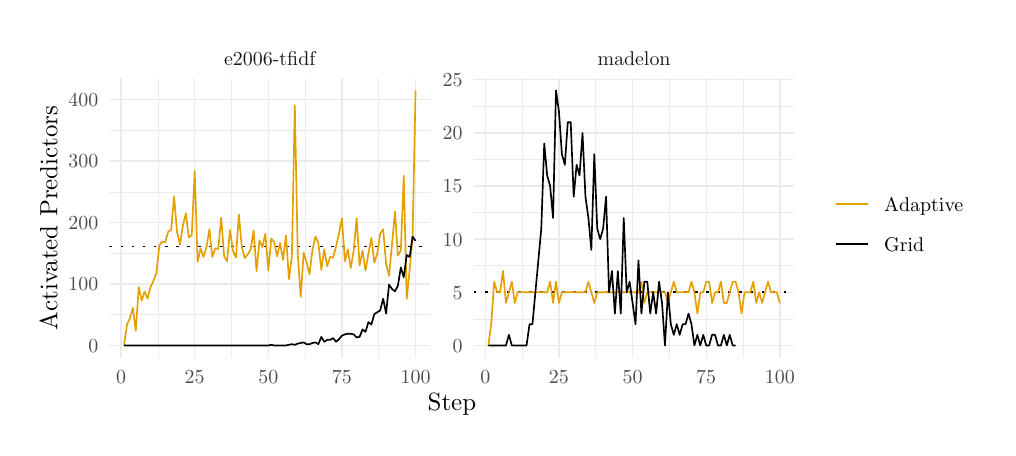
\begin{tikzpicture}[x=1pt,y=1pt]
\definecolor{fillColor}{RGB}{255,255,255}
\path[use as bounding box,fill=fillColor,fill opacity=0.00] (0,0) rectangle (346.90,144.54);
\begin{scope}
\path[clip] ( 29.55, 25.11) rectangle (145.42,126.48);
\definecolor{drawColor}{gray}{0.92}

\path[draw=drawColor,line width= 0.2pt,line join=round] ( 29.55, 40.82) --
	(145.42, 40.82);

\path[draw=drawColor,line width= 0.2pt,line join=round] ( 29.55, 63.02) --
	(145.42, 63.02);

\path[draw=drawColor,line width= 0.2pt,line join=round] ( 29.55, 85.23) --
	(145.42, 85.23);

\path[draw=drawColor,line width= 0.2pt,line join=round] ( 29.55,107.44) --
	(145.42,107.44);

\path[draw=drawColor,line width= 0.2pt,line join=round] ( 47.05, 25.11) --
	( 47.05,126.48);

\path[draw=drawColor,line width= 0.2pt,line join=round] ( 73.65, 25.11) --
	( 73.65,126.48);

\path[draw=drawColor,line width= 0.2pt,line join=round] (100.25, 25.11) --
	(100.25,126.48);

\path[draw=drawColor,line width= 0.2pt,line join=round] (126.85, 25.11) --
	(126.85,126.48);

\path[draw=drawColor,line width= 0.5pt,line join=round] ( 29.55, 29.71) --
	(145.42, 29.71);

\path[draw=drawColor,line width= 0.5pt,line join=round] ( 29.55, 51.92) --
	(145.42, 51.92);

\path[draw=drawColor,line width= 0.5pt,line join=round] ( 29.55, 74.13) --
	(145.42, 74.13);

\path[draw=drawColor,line width= 0.5pt,line join=round] ( 29.55, 96.34) --
	(145.42, 96.34);

\path[draw=drawColor,line width= 0.5pt,line join=round] ( 29.55,118.54) --
	(145.42,118.54);

\path[draw=drawColor,line width= 0.5pt,line join=round] ( 33.75, 25.11) --
	( 33.75,126.48);

\path[draw=drawColor,line width= 0.5pt,line join=round] ( 60.35, 25.11) --
	( 60.35,126.48);

\path[draw=drawColor,line width= 0.5pt,line join=round] ( 86.95, 25.11) --
	( 86.95,126.48);

\path[draw=drawColor,line width= 0.5pt,line join=round] (113.55, 25.11) --
	(113.55,126.48);

\path[draw=drawColor,line width= 0.5pt,line join=round] (140.16, 25.11) --
	(140.16,126.48);
\definecolor{drawColor}{RGB}{0,0,0}

\path[draw=drawColor,line width= 0.6pt,dash pattern=on 1pt off 3pt ,line join=round] ( 29.55, 65.44) -- (145.42, 65.44);
\definecolor{drawColor}{RGB}{230,159,0}

\path[draw=drawColor,line width= 0.6pt,line join=round] ( 34.81, 29.71) --
	( 35.88, 37.26) --
	( 36.94, 39.49) --
	( 38.00, 43.26) --
	( 39.07, 35.04) --
	( 40.13, 50.81) --
	( 41.20, 45.93) --
	( 42.26, 49.26) --
	( 43.33, 46.59) --
	( 44.39, 50.81) --
	( 45.45, 53.03) --
	( 46.52, 55.92) --
	( 47.58, 65.91) --
	( 48.65, 67.24) --
	( 49.71, 67.02) --
	( 50.77, 70.80) --
	( 51.84, 71.46) --
	( 52.90, 83.46) --
	( 53.97, 70.80) --
	( 55.03, 66.13) --
	( 56.09, 73.02) --
	( 57.16, 77.46) --
	( 58.22, 68.80) --
	( 59.29, 69.46) --
	( 60.35, 92.78) --
	( 61.41, 59.92) --
	( 62.48, 64.80) --
	( 63.54, 61.69) --
	( 64.61, 65.25) --
	( 65.67, 71.69) --
	( 66.73, 61.69) --
	( 67.80, 64.80) --
	( 68.86, 64.58) --
	( 69.93, 75.91) --
	( 70.99, 61.91) --
	( 72.06, 60.14) --
	( 73.12, 71.46) --
	( 74.18, 63.91) --
	( 75.25, 61.47) --
	( 76.31, 77.02) --
	( 77.38, 65.25) --
	( 78.44, 61.25) --
	( 79.50, 62.58) --
	( 80.57, 64.36) --
	( 81.63, 71.24) --
	( 82.70, 56.58) --
	( 83.76, 67.69) --
	( 84.82, 65.25) --
	( 85.89, 70.13) --
	( 86.95, 56.81) --
	( 88.02, 68.35) --
	( 89.08, 67.02) --
	( 90.14, 61.91) --
	( 91.21, 66.80) --
	( 92.27, 60.58) --
	( 93.34, 69.46) --
	( 94.40, 53.70) --
	( 95.46, 61.91) --
	( 96.53,116.54) --
	( 97.59, 62.80) --
	( 98.66, 47.26) --
	( 99.72, 63.25) --
	(100.79, 59.69) --
	(101.85, 55.47) --
	(102.91, 64.36) --
	(103.98, 69.02) --
	(105.04, 66.80) --
	(106.11, 57.03) --
	(107.17, 64.36) --
	(108.23, 58.36) --
	(109.30, 61.69) --
	(110.36, 61.47) --
	(111.43, 65.47) --
	(112.49, 70.13) --
	(113.55, 75.68) --
	(114.62, 60.14) --
	(115.68, 64.36) --
	(116.75, 57.70) --
	(117.81, 64.14) --
	(118.87, 75.68) --
	(119.94, 58.58) --
	(121.00, 63.91) --
	(122.07, 56.81) --
	(123.13, 63.02) --
	(124.19, 68.58) --
	(125.26, 59.69) --
	(126.32, 62.80) --
	(127.39, 70.13) --
	(128.45, 71.69) --
	(129.52, 59.25) --
	(130.58, 54.81) --
	(131.64, 66.13) --
	(132.71, 78.13) --
	(133.77, 62.14) --
	(134.84, 64.14) --
	(135.90, 91.01) --
	(136.96, 46.59) --
	(138.03, 57.03) --
	(139.09, 69.24) --
	(140.16,121.87);
\definecolor{drawColor}{RGB}{0,0,0}

\path[draw=drawColor,line width= 0.6pt,line join=round] ( 34.81, 29.71) --
	( 35.88, 29.71) --
	( 36.94, 29.71) --
	( 38.00, 29.71) --
	( 39.07, 29.71) --
	( 40.13, 29.71) --
	( 41.20, 29.71) --
	( 42.26, 29.71) --
	( 43.33, 29.71) --
	( 44.39, 29.71) --
	( 45.45, 29.71) --
	( 46.52, 29.71) --
	( 47.58, 29.71) --
	( 48.65, 29.71) --
	( 49.71, 29.71) --
	( 50.77, 29.71) --
	( 51.84, 29.71) --
	( 52.90, 29.71) --
	( 53.97, 29.71) --
	( 55.03, 29.71) --
	( 56.09, 29.71) --
	( 57.16, 29.71) --
	( 58.22, 29.71) --
	( 59.29, 29.71) --
	( 60.35, 29.71) --
	( 61.41, 29.71) --
	( 62.48, 29.71) --
	( 63.54, 29.71) --
	( 64.61, 29.71) --
	( 65.67, 29.71) --
	( 66.73, 29.71) --
	( 67.80, 29.71) --
	( 68.86, 29.71) --
	( 69.93, 29.71) --
	( 70.99, 29.71) --
	( 72.06, 29.71) --
	( 73.12, 29.71) --
	( 74.18, 29.71) --
	( 75.25, 29.71) --
	( 76.31, 29.71) --
	( 77.38, 29.71) --
	( 78.44, 29.71) --
	( 79.50, 29.71) --
	( 80.57, 29.71) --
	( 81.63, 29.71) --
	( 82.70, 29.71) --
	( 83.76, 29.71) --
	( 84.82, 29.71) --
	( 85.89, 29.71) --
	( 86.95, 29.71) --
	( 88.02, 29.94) --
	( 89.08, 29.71) --
	( 90.14, 29.71) --
	( 91.21, 29.71) --
	( 92.27, 29.71) --
	( 93.34, 29.71) --
	( 94.40, 29.94) --
	( 95.46, 30.16) --
	( 96.53, 29.94) --
	( 97.59, 30.38) --
	( 98.66, 30.60) --
	( 99.72, 30.82) --
	(100.79, 30.16) --
	(101.85, 30.16) --
	(102.91, 30.60) --
	(103.98, 30.82) --
	(105.04, 30.16) --
	(106.11, 32.82) --
	(107.17, 31.05) --
	(108.23, 31.71) --
	(109.30, 31.71) --
	(110.36, 32.38) --
	(111.43, 31.05) --
	(112.49, 31.94) --
	(113.55, 33.27) --
	(114.62, 33.71) --
	(115.68, 33.93) --
	(116.75, 33.93) --
	(117.81, 33.71) --
	(118.87, 32.60) --
	(119.94, 32.82) --
	(121.00, 35.49) --
	(122.07, 34.60) --
	(123.13, 38.15) --
	(124.19, 37.26) --
	(125.26, 41.04) --
	(126.32, 41.71) --
	(127.39, 42.37) --
	(128.45, 46.59) --
	(129.52, 41.26) --
	(130.58, 51.70) --
	(131.64, 50.14) --
	(132.71, 49.26) --
	(133.77, 51.26) --
	(134.84, 57.92) --
	(135.90, 54.36) --
	(136.96, 62.36) --
	(138.03, 61.69) --
	(139.09, 69.02) --
	(140.16, 67.47);
\end{scope}
\begin{scope}
\path[clip] (161.17, 25.11) rectangle (277.05,126.48);
\definecolor{drawColor}{gray}{0.92}

\path[draw=drawColor,line width= 0.2pt,line join=round] (161.17, 39.31) --
	(277.05, 39.31);

\path[draw=drawColor,line width= 0.2pt,line join=round] (161.17, 58.51) --
	(277.05, 58.51);

\path[draw=drawColor,line width= 0.2pt,line join=round] (161.17, 77.71) --
	(277.05, 77.71);

\path[draw=drawColor,line width= 0.2pt,line join=round] (161.17, 96.91) --
	(277.05, 96.91);

\path[draw=drawColor,line width= 0.2pt,line join=round] (161.17,116.11) --
	(277.05,116.11);

\path[draw=drawColor,line width= 0.2pt,line join=round] (178.68, 25.11) --
	(178.68,126.48);

\path[draw=drawColor,line width= 0.2pt,line join=round] (205.28, 25.11) --
	(205.28,126.48);

\path[draw=drawColor,line width= 0.2pt,line join=round] (231.88, 25.11) --
	(231.88,126.48);

\path[draw=drawColor,line width= 0.2pt,line join=round] (258.48, 25.11) --
	(258.48,126.48);

\path[draw=drawColor,line width= 0.5pt,line join=round] (161.17, 29.71) --
	(277.05, 29.71);

\path[draw=drawColor,line width= 0.5pt,line join=round] (161.17, 48.91) --
	(277.05, 48.91);

\path[draw=drawColor,line width= 0.5pt,line join=round] (161.17, 68.11) --
	(277.05, 68.11);

\path[draw=drawColor,line width= 0.5pt,line join=round] (161.17, 87.31) --
	(277.05, 87.31);

\path[draw=drawColor,line width= 0.5pt,line join=round] (161.17,106.51) --
	(277.05,106.51);

\path[draw=drawColor,line width= 0.5pt,line join=round] (161.17,125.71) --
	(277.05,125.71);

\path[draw=drawColor,line width= 0.5pt,line join=round] (165.37, 25.11) --
	(165.37,126.48);

\path[draw=drawColor,line width= 0.5pt,line join=round] (191.98, 25.11) --
	(191.98,126.48);

\path[draw=drawColor,line width= 0.5pt,line join=round] (218.58, 25.11) --
	(218.58,126.48);

\path[draw=drawColor,line width= 0.5pt,line join=round] (245.18, 25.11) --
	(245.18,126.48);

\path[draw=drawColor,line width= 0.5pt,line join=round] (271.78, 25.11) --
	(271.78,126.48);
\definecolor{drawColor}{RGB}{0,0,0}

\path[draw=drawColor,line width= 0.6pt,dash pattern=on 1pt off 3pt ,line join=round] (161.17, 48.91) -- (277.05, 48.91);
\definecolor{drawColor}{RGB}{230,159,0}

\path[draw=drawColor,line width= 0.6pt,line join=round] (166.44, 29.71) --
	(167.50, 37.39) --
	(168.57, 52.75) --
	(169.63, 48.91) --
	(170.69, 48.91) --
	(171.76, 56.59) --
	(172.82, 45.07) --
	(173.89, 48.91) --
	(174.95, 52.75) --
	(176.02, 45.07) --
	(177.08, 48.91) --
	(178.14, 48.91) --
	(179.21, 48.91) --
	(180.27, 48.91) --
	(181.34, 48.91) --
	(182.40, 48.91) --
	(183.46, 48.91) --
	(184.53, 48.91) --
	(185.59, 48.91) --
	(186.66, 48.91) --
	(187.72, 48.91) --
	(188.78, 52.75) --
	(189.85, 45.07) --
	(190.91, 52.75) --
	(191.98, 45.07) --
	(193.04, 48.91) --
	(194.10, 48.91) --
	(195.17, 48.91) --
	(196.23, 48.91) --
	(197.30, 48.91) --
	(198.36, 48.91) --
	(199.42, 48.91) --
	(200.49, 48.91) --
	(201.55, 48.91) --
	(202.62, 52.75) --
	(203.68, 48.91) --
	(204.75, 45.07) --
	(205.81, 48.91) --
	(206.87, 48.91) --
	(207.94, 48.91) --
	(209.00, 48.91) --
	(210.07, 48.91) --
	(211.13, 48.91) --
	(212.19, 48.91) --
	(213.26, 48.91) --
	(214.32, 48.91) --
	(215.39, 48.91) --
	(216.45, 48.91) --
	(217.51, 48.91) --
	(218.58, 48.91) --
	(219.64, 48.91) --
	(220.71, 48.91) --
	(221.77, 52.75) --
	(222.83, 45.07) --
	(223.90, 48.91) --
	(224.96, 48.91) --
	(226.03, 48.91) --
	(227.09, 48.91) --
	(228.15, 48.91) --
	(229.22, 48.91) --
	(230.28, 48.91) --
	(231.35, 45.07) --
	(232.41, 48.91) --
	(233.48, 52.75) --
	(234.54, 48.91) --
	(235.60, 48.91) --
	(236.67, 48.91) --
	(237.73, 48.91) --
	(238.80, 48.91) --
	(239.86, 52.75) --
	(240.92, 48.91) --
	(241.99, 41.23) --
	(243.05, 48.91) --
	(244.12, 48.91) --
	(245.18, 52.75) --
	(246.24, 52.75) --
	(247.31, 45.07) --
	(248.37, 48.91) --
	(249.44, 48.91) --
	(250.50, 52.75) --
	(251.56, 45.07) --
	(252.63, 45.07) --
	(253.69, 48.91) --
	(254.76, 52.75) --
	(255.82, 52.75) --
	(256.88, 48.91) --
	(257.95, 41.23) --
	(259.01, 48.91) --
	(260.08, 48.91) --
	(261.14, 48.91) --
	(262.21, 52.75) --
	(263.27, 45.07) --
	(264.33, 48.91) --
	(265.40, 45.07) --
	(266.46, 48.91) --
	(267.53, 52.75) --
	(268.59, 48.91) --
	(269.65, 48.91) --
	(270.72, 48.91) --
	(271.78, 45.07);
\definecolor{drawColor}{RGB}{0,0,0}

\path[draw=drawColor,line width= 0.6pt,line join=round] (166.44, 29.71) --
	(167.50, 29.71) --
	(168.57, 29.71) --
	(169.63, 29.71) --
	(170.69, 29.71) --
	(171.76, 29.71) --
	(172.82, 29.71) --
	(173.89, 33.55) --
	(174.95, 29.71) --
	(176.02, 29.71) --
	(177.08, 29.71) --
	(178.14, 29.71) --
	(179.21, 29.71) --
	(180.27, 29.71) --
	(181.34, 37.39) --
	(182.40, 37.39) --
	(183.46, 48.91) --
	(184.53, 60.43) --
	(185.59, 71.95) --
	(186.66,102.67) --
	(187.72, 91.15) --
	(188.78, 87.31) --
	(189.85, 75.79) --
	(190.91,121.87) --
	(191.98,114.19) --
	(193.04, 98.83) --
	(194.10, 94.99) --
	(195.17,110.35) --
	(196.23,110.35) --
	(197.30, 83.47) --
	(198.36, 94.99) --
	(199.42, 91.15) --
	(200.49,106.51) --
	(201.55, 83.47) --
	(202.62, 75.79) --
	(203.68, 64.27) --
	(204.75, 98.83) --
	(205.81, 71.95) --
	(206.87, 68.11) --
	(207.94, 71.95) --
	(209.00, 83.47) --
	(210.07, 48.91) --
	(211.13, 56.59) --
	(212.19, 41.23) --
	(213.26, 56.59) --
	(214.32, 41.23) --
	(215.39, 75.79) --
	(216.45, 48.91) --
	(217.51, 52.75) --
	(218.58, 45.07) --
	(219.64, 37.39) --
	(220.71, 60.43) --
	(221.77, 41.23) --
	(222.83, 52.75) --
	(223.90, 52.75) --
	(224.96, 41.23) --
	(226.03, 48.91) --
	(227.09, 41.23) --
	(228.15, 52.75) --
	(229.22, 45.07) --
	(230.28, 29.71) --
	(231.35, 48.91) --
	(232.41, 37.39) --
	(233.48, 33.55) --
	(234.54, 37.39) --
	(235.60, 33.55) --
	(236.67, 37.39) --
	(237.73, 37.39) --
	(238.80, 41.23) --
	(239.86, 37.39) --
	(240.92, 29.71) --
	(241.99, 33.55) --
	(243.05, 29.71) --
	(244.12, 33.55) --
	(245.18, 29.71) --
	(246.24, 29.71) --
	(247.31, 33.55) --
	(248.37, 33.55) --
	(249.44, 29.71) --
	(250.50, 29.71) --
	(251.56, 33.55) --
	(252.63, 29.71) --
	(253.69, 33.55) --
	(254.76, 29.71) --
	(255.82, 29.71);
\end{scope}
\begin{scope}
\path[clip] ( 29.55,126.48) rectangle (145.42,140.04);
\definecolor{drawColor}{gray}{0.10}

\node[text=drawColor,anchor=base,inner sep=0pt, outer sep=0pt, scale=  0.72] at ( 87.48,130.78) {e2006-tfidf};
\end{scope}
\begin{scope}
\path[clip] (161.17,126.48) rectangle (277.05,140.04);
\definecolor{drawColor}{gray}{0.10}

\node[text=drawColor,anchor=base,inner sep=0pt, outer sep=0pt, scale=  0.72] at (219.11,130.78) {madelon};
\end{scope}
\begin{scope}
\path[clip] (  0.00,  0.00) rectangle (346.90,144.54);
\definecolor{drawColor}{gray}{0.30}

\node[text=drawColor,anchor=base,inner sep=0pt, outer sep=0pt, scale=  0.72] at ( 33.75, 16.10) {0};

\node[text=drawColor,anchor=base,inner sep=0pt, outer sep=0pt, scale=  0.72] at ( 60.35, 16.10) {25};

\node[text=drawColor,anchor=base,inner sep=0pt, outer sep=0pt, scale=  0.72] at ( 86.95, 16.10) {50};

\node[text=drawColor,anchor=base,inner sep=0pt, outer sep=0pt, scale=  0.72] at (113.55, 16.10) {75};

\node[text=drawColor,anchor=base,inner sep=0pt, outer sep=0pt, scale=  0.72] at (140.16, 16.10) {100};
\end{scope}
\begin{scope}
\path[clip] (  0.00,  0.00) rectangle (346.90,144.54);
\definecolor{drawColor}{gray}{0.30}

\node[text=drawColor,anchor=base,inner sep=0pt, outer sep=0pt, scale=  0.72] at (165.37, 16.10) {0};

\node[text=drawColor,anchor=base,inner sep=0pt, outer sep=0pt, scale=  0.72] at (191.98, 16.10) {25};

\node[text=drawColor,anchor=base,inner sep=0pt, outer sep=0pt, scale=  0.72] at (218.58, 16.10) {50};

\node[text=drawColor,anchor=base,inner sep=0pt, outer sep=0pt, scale=  0.72] at (245.18, 16.10) {75};

\node[text=drawColor,anchor=base,inner sep=0pt, outer sep=0pt, scale=  0.72] at (271.78, 16.10) {100};
\end{scope}
\begin{scope}
\path[clip] (  0.00,  0.00) rectangle (346.90,144.54);
\definecolor{drawColor}{gray}{0.30}

\node[text=drawColor,anchor=base east,inner sep=0pt, outer sep=0pt, scale=  0.72] at (157.12, 27.24) {0};

\node[text=drawColor,anchor=base east,inner sep=0pt, outer sep=0pt, scale=  0.72] at (157.12, 46.43) {5};

\node[text=drawColor,anchor=base east,inner sep=0pt, outer sep=0pt, scale=  0.72] at (157.12, 65.63) {10};

\node[text=drawColor,anchor=base east,inner sep=0pt, outer sep=0pt, scale=  0.72] at (157.12, 84.83) {15};

\node[text=drawColor,anchor=base east,inner sep=0pt, outer sep=0pt, scale=  0.72] at (157.12,104.03) {20};

\node[text=drawColor,anchor=base east,inner sep=0pt, outer sep=0pt, scale=  0.72] at (157.12,123.23) {25};
\end{scope}
\begin{scope}
\path[clip] (  0.00,  0.00) rectangle (346.90,144.54);
\definecolor{drawColor}{gray}{0.30}

\node[text=drawColor,anchor=base east,inner sep=0pt, outer sep=0pt, scale=  0.72] at ( 25.50, 27.24) {0};

\node[text=drawColor,anchor=base east,inner sep=0pt, outer sep=0pt, scale=  0.72] at ( 25.50, 49.44) {100};

\node[text=drawColor,anchor=base east,inner sep=0pt, outer sep=0pt, scale=  0.72] at ( 25.50, 71.65) {200};

\node[text=drawColor,anchor=base east,inner sep=0pt, outer sep=0pt, scale=  0.72] at ( 25.50, 93.86) {300};

\node[text=drawColor,anchor=base east,inner sep=0pt, outer sep=0pt, scale=  0.72] at ( 25.50,116.06) {400};
\end{scope}
\begin{scope}
\path[clip] (  0.00,  0.00) rectangle (346.90,144.54);
\definecolor{drawColor}{RGB}{0,0,0}

\node[text=drawColor,anchor=base,inner sep=0pt, outer sep=0pt, scale=  0.90] at (153.30,  6.25) {Step};
\end{scope}
\begin{scope}
\path[clip] (  0.00,  0.00) rectangle (346.90,144.54);
\definecolor{drawColor}{RGB}{0,0,0}

\node[text=drawColor,rotate= 90.00,anchor=base,inner sep=0pt, outer sep=0pt, scale=  0.90] at ( 10.70, 75.79) {Activated Predictors};
\end{scope}
\begin{scope}
\path[clip] (  0.00,  0.00) rectangle (346.90,144.54);
\definecolor{drawColor}{RGB}{230,159,0}

\path[draw=drawColor,line width= 0.6pt,line join=round] (291.99, 80.77) -- (303.56, 80.77);
\end{scope}
\begin{scope}
\path[clip] (  0.00,  0.00) rectangle (346.90,144.54);
\definecolor{drawColor}{RGB}{0,0,0}

\path[draw=drawColor,line width= 0.6pt,line join=round] (291.99, 66.32) -- (303.56, 66.32);
\end{scope}
\begin{scope}
\path[clip] (  0.00,  0.00) rectangle (346.90,144.54);
\definecolor{drawColor}{RGB}{0,0,0}

\node[text=drawColor,anchor=base west,inner sep=0pt, outer sep=0pt, scale=  0.72] at (309.50, 78.29) {Adaptive};
\end{scope}
\begin{scope}
\path[clip] (  0.00,  0.00) rectangle (346.90,144.54);
\definecolor{drawColor}{RGB}{0,0,0}

\node[text=drawColor,anchor=base west,inner sep=0pt, outer sep=0pt, scale=  0.72] at (309.50, 63.84) {Grid};
\end{scope}
\end{tikzpicture}
